\documentclass{article}



\usepackage{arxiv}

\usepackage[utf8]{inputenc} % allow utf-8 input
\usepackage[T1]{fontenc}    % use 8-bit T1 fonts
\usepackage{hyperref}       % hyperlinks
\usepackage{amsfonts}       % blackboard math symbols
\usepackage{amsthm}
\usepackage{amsmath}
\usepackage{amssymb}
\usepackage{float}
\theoremstyle{definition}
\newtheorem{example}{Example}
%\newtheorem{assumption}{Assumption}
\theoremstyle{theorem}
\newtheorem{proposition}{Proposition}

\numberwithin{proposition}{section}
\usepackage{graphicx}
%REMOVE IN THE FUTURE
\usepackage{xcolor}


\title{Two-dimensional strip packing problem}


%\author{ }

\date{}



%%% Add PDF metadata to help others organize their library
%%% Once the PDF is generated, you can check the metadata with
%%% $ pdfinfo template.pdf
%\hypersetup{}

\begin{document}
\maketitle
\section*{Introduction}
    In 1980, B. S. Baker and E. G. Coffman proposed the problem \cite{bakercoffmanrivest}: Given a vertical strip of width $W$, bounded below but not above, and a list $L$ of rectangular regions $R_1\dots R_n$, pack the regions into the strip so that the final height is a minimal. We also assume each region $R_i$, $1\leq i \leq n$, is to be defined by its width $w_i$ and height $h_i$. The rectangles are allowed neither to overlap nor to rotate. This type of packing is called a \textit{two-dimensional strip packing}.
\section*{Definition}
    Let us consider the vertical strip
    \begin{equation*}
        S=\{(x,y)\in\mathbb{Q}^2\mid0\leq x\leq W,~y\geq 0\},~W\in\mathbb{Q}_{+}
    \end{equation*}
    and the list $L=\{(w_i,h_i)\}^{n}_{i=1}\subset\mathbb{Q}^2_{+}$, $n\in\mathbb{N}$. Let also $O:=\{(x_i,y_i)\}_{i=1}^{n}\subset\mathbb{Q}^2$ and $R_i:=[x_i;x_i+w_i]\times[y_i;y_i+h_i]\cap\mathbb{Q}^2$. Let us note that elements of $L$ can duplicate. 

    A pair $P=(S,R)$, $R=\{R_i\}_{i=1}^{n}$, is called a \textit{strip packing w.r.t. $S$ and $L$} if the following conditions hold
    \begin{enumerate}
        \item
        $R_i\subset S$, for any $i$, $1\leq i\leq n$.
        \item
        ${\rm Int}(R_i)\cap{\rm Int}(R_j)=\varnothing$, for any $i,j$, $1\leq i,j\leq n$, $i\neq j$. 
    \end{enumerate} 
    Here ${\rm Int}(R_i):=(x_i;x_{i}+w_i)\times(y_i;y_i+h_i)\cap\mathbb{Q}^2$. 

    A value 
    \begin{equation*}
        H(P):=\max_{1\leq i\leq n}(y_i+h_i)
    \end{equation*}
    is called a \textit{height} of strip packing $P$.

    Let $\mathcal{P}$ be a family of all strip packings w.r.t. $S$ and $L$. A packing $P^{*}\in\mathcal{P}$ is called \textit{optimal} if it satisfies the optimum condition
    \begin{equation*}
        H(P^{*})=\min_{P\in\mathcal{P}}H(P).
    \end{equation*}
    A height $H^{*}:=H(P^{*})$ is called an \textit{optimal height}. 

    The objective of the \textit{strip packing problem} is to find $P^{*}$. This problem is strongly NP-hard. 

    There are numerous ways to model and solve this problem (see \cite{lodimartellomonaci}). We will focus on the Steinberg approximation algorithm and two heuristics.
\section*{Steinberg algorithm}
    Let us focus on the Steinberg algorithm. See \cite{steinberg}. It is an example of approximating algorithms with a predefined ratio of the upper bound. That is, there is $\alpha>1$ such that
    \begin{equation*}
        \tilde{H}\leq \alpha H^{*},
    \end{equation*}
    where $\tilde{H}$ stands for the height obtained with the algorithm.


    For the Steinberg approximation, $\alpha=2$. Nowadays, the best algorithm provides $\alpha = \frac{5}{4} + \varepsilon$ \cite{jansenrau}.

    At the end of this section, we also provide two simple modifications of the Steinberg algorithm and obtain empirical ratios for them. Let
    \begin{equation*}
        S=\{(x,y)\in\mathbb{Q}^2\mid 0\leq x\leq W,~y\geq 0\},~W\in\mathbb{Q}_{+},
    \end{equation*}
    and
    \begin{equation*}
        L=\{(w_i,h_i)\}_{i=1}^{n}\in \mathbb{Q}^2_{+},~n\in\mathbb{N}.
    \end{equation*}
 
    Let $S = \sum w_ih_i$, $w = \max\{w_i\}$, $h = \max\{h_i\}$.

    The Steinberg algorithm provides packing into a container 
    \begin{equation*}
        Q=[0;W]\times[0;H]\cap \mathbb{Q}^2,~W,H\in\mathbb{Q}_{+}
    \end{equation*}
    where $W, H$ satisfy the conditions
    \begin{equation*}
        w\leq W,~h\leq H,~2S\leq WH-\max\{2w-W,0\}\cdot \max\{2h-H,0\}.
    \end{equation*}
    If these conditions hold, then there exists the Steinberg packing.

    For any rectangle $R = [x_1; x_2]\times [y_1; y_2]\cap Q^2$, let us provide the notations
    \begin{equation*}
        {}_{*}[R]: = (x_1, y_1),~{}^{*}[R]: = (x_1, y_2),~[R]_{*}: = (x_2, y_1),~[R]^{*}: = (x_2, y_2) 
    \end{equation*}
    The Steinberg algorithms is the following:

    \textbf{Step 1} We need to compute $H$ to satisfy sufficient conditions. Put $H := \max\{H', h\}$, where
    \begin{equation*}
        H':=\begin{cases}
            \frac{S+4wh-Wh}{2w} & S \leq Wh \leq 2wh\\
            \frac{2S}{W} & \text{otherwise}
        \end{cases}
    \end{equation*}
    \textbf{Step 2} We recursively perform the reduction process for $Q$ and $L$. The process then stops after packing all rectangles. Given an arbitrary $(Q, L)$, we use an appropriate procedure from the following list
    \begin{enumerate}
        \item[\textbf{\textit{P1}}] 
            This procedure can be applied to the $(Q, L)$ if the condition holds: 
            \begin{equation*}
                2w \geq W
            \end{equation*}
            First, we order and re-number the rectangles of list $L$ by decreasing width $w_1 \geq\dots\geq w_n$. Let $m$, $1\leq m\leq n$, be the maximal index such that $2w_m\geq W$. Place the rectangles $R_1,\dots,R_m$ so that
            \begin{equation*}
                {}_{*}[R_1]={}_{*}[Q]~\text{and}~{}_{*}[R_i]={}^{*}[R_{i-1}],~2\leq i\leq m
            \end{equation*}
            If $m = n$, procedure P1 solves the problem. Suppose that $m < n$. Let
            \begin{equation*}
                h' =H-\sum_{i=1}^{m}h_i.
            \end{equation*}
            We order and re-number the rectangles $R_{m+1},\dots,R_n$ by decreasing height $h_{m+1}\geq\dots\geq h_n$. 

            If $h_{m+1}\leq h'$, we form a problem $(Q',L')$, where $L' = \{(w_i,h_i)\}_{i=m+1}^{n}$ and the container $Q'$ is defined as
            \begin{equation*}
                {}_{*}[Q'] = {}^{*}[R_m],~[Q']^{*} = [Q]^{*}
            \end{equation*}

            If $h_{m+1} >h'$, denote by $k$, $m+1\leq k\leq n$, the maximal index for which $b_k>h'$ and place $R_{m+1},\dots,R_k$ in the following way
            \begin{equation*}
                [R_1]^{*} =[Q]^{*}~\text{and}~[R_i]^{*}={}^{*}[R_{i-1}],~m+2\leq i\leq k
            \end{equation*}
            If $k=n$, procedure P1 solves the problem. Suppose that $k < n$, we form a problem $(Q', L')$, where $L' = \{(w_i, h_i)\}_{i=k+1}^{n}$ and the container $Q'$ is defined as
            \begin{equation*}
                {}_{*}[Q'] = {}^{*}[R_m],~[Q']^{*} = {}^{*}[R_k] 
            \end{equation*}
        \item[\textbf{\textit{Pm1}}]
            This procedure can be applied to the $(Q, L)$ if the condition holds: 
            \begin{equation*}
                2h \geq H
            \end{equation*}
            This procedure is transformed from P1 by interchanging the horizontal and vertical directions.
        \item[\textbf{\textit{P3}}]
            First, we order and re-number the rectangles of list $L$ by decreasing width $w_1 \geq\dots\geq  w_n$.

            This procedure can be applied to the $(Q, L)$ if the conditions hold: 
            \begin{equation*}
                2w\leq W,~2h\leq H,~n>1,
            \end{equation*}
            and
            \begin{equation*}
                S-\frac{1}{4}WH\leq \sum_{i=1}^{m}w_ih_i \leq \frac{3}{8}WH,~w_{m+1}\leq\frac{1}{4}W,
            \end{equation*}
            for some index $m$, $1 \leq m < n$.

            We set $W' := \max\{\frac{1}{2}W, \frac{2\sum_{i=1}^{n}w_ih_i}{H}\}$, $W'' := W - W'$. Then we cut $Q$ into two containers $Q'$ and $Q''$ with widths $W'$ and $W''$ and the same height $H$, and we consider now two problems $(Q', L')$ and $(Q'', L'')$ with $L' = \{(w_i, h_i)\}_{i=1}^{m}$, $L'' = \{(w_i, h_i)\}_{i=m+1}^{n}$.
        \item[\textbf{\textit{Pm3}}]
            First, we order and re-number the rectangles of list $L$ by decreasing height $h_1 \geq\dots\geq h_n$. 

            This procedure can be applied to the $(Q, L)$ if the conditions hold:
            \begin{equation*}
                2w\leq W,~2h\leq H,~n>1,
            \end{equation*}
            and 
            \begin{equation*}
                S-\frac{1}{4}WH\leq \sum_{i=1}^{m}w_ih_i\leq \frac{3}{8}WH,~h_{m+1}\leq\frac{1}{4}H
            \end{equation*}
            for some index $m$, $1 \leq m < n$.

            This procedure is transformed from P3 by interchanging the horizontal and vertical directions.
        \item[\textbf{\textit{P2}}]
            This procedure can be applied to the $(Q, L)$ if the conditions hold: 
            \begin{equation*}
                2w\leq W,~2h\leq H,~n>1,
            \end{equation*}
            and there exist two different indices $i$ and $k$ such that
            \begin{equation*}
                w_i,w_k \geq \frac{1}{4}W,~h_i,h_k \geq \frac{1}{4}H,~2(S-w_i\cdot h_i - w_k\cdot h_k)\leq (W - \max\{w_i,w_k\})H.
            \end{equation*}
            Assuming that $w_i \geq w_k$, we place $R_i$ and $R_k$ so that 
            \begin{equation*}
                {}_{*}[R_i] = {}_{*}[Q],~{}_{*}[R_k] = {}^{*}[R_i].
            \end{equation*}
            If $n > 2$, we consider a new problem $(Q',L')$, where $L' = L\setminus\{(w_i,h_i), (w_k,h_k)\}$ and $Q'$ is the container such that
            \begin{equation*}
                {}_{*}[Q'] = [R_i]_{*},~[Q']^{*} = [Q]^{*}.
            \end{equation*}
        \item[\textbf{\textit{Pm2}}]
            This procedure can be applied to the $(Q, L)$ if the conditions hold: 
            \begin{equation*}
                2w\leq W,~2h\leq H,~n>1,
            \end{equation*}
            and there exist two different indices $i$ and $k$ such that
            \begin{equation*}
                w_i,w_k \geq \frac{1}{4}W,~h_i,h_k \geq \frac{1}{4}H,~2(S-w_i\cdot h_i -w_k\cdot h_k)\leq (H-\max\{h_i,h_k\})W.
            \end{equation*}
            This procedure is transformed from P2 by interchanging the horizontal and vertical directions.
        \item[\textbf{\textit{P0}}]
            This procedure can be applied to the $(Q, L)$ if the (remaining) conditions hold:
            \begin{equation*}
                2w\leq W,~2h\leq H,~\text{and}~S-\frac{1}{4}WH\leq w_ih_i
            \end{equation*}
            for some index $i$, $1 \leq i \leq n$.

            We place $R_i$ so that
            \begin{equation*}
                 {}_{*}[R_i] = {}_{*}[Q].
            \end{equation*}
            If $n>1$, we consider a new problem $(Q',L')$, where $L' = L \setminus \{(w_i,h_i)\}$ and $Q'$ is the container such that
            \begin{equation*}
                {}_{*}[Q']=[R_i]_{*},~[Q']^{*}=[Q]^{*}.
            \end{equation*}
    \end{enumerate}
    The Steinberg algorithm time complexity is $O(\frac{n\log^2 n}{\log\log n})$. 
\section*{Examples}
    \begin{example}\label{ex1}
        Let $W = 2$ and $L = \{(1,1),~(1,1),~(2,1)\}$. Obviously, $H^{*} = 2$. Steinberg’s packing provides $H = 3 > H^{*}$. Respective packing is pictured below
        \begin{figure}[H]
            \centering
            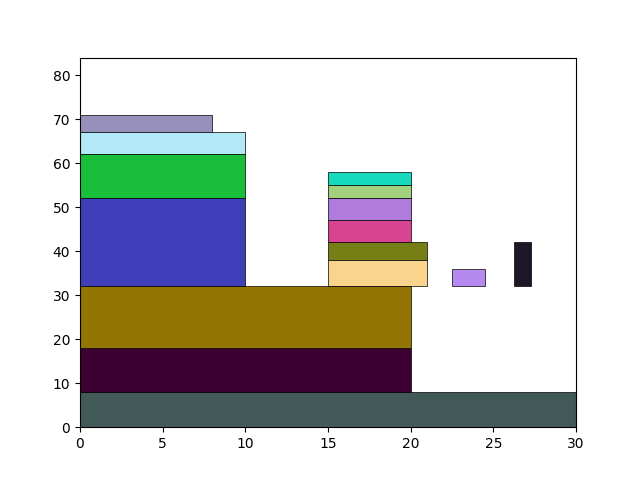
\includegraphics[scale=0.5]{../examples/original-1.png}
            \caption{Example \ref{ex1}, original Steinberg algorithm}
        \end{figure} 
    \end{example}
    \begin{example}\label{ex2}
        Let $W = 30$ and $L = \{(20, 6),~(3, 10),~(7, 10),~(20, 12),~(10, 8),~(30, 10)\}$. We have that $H^{*} = 28$:
        \begin{equation*}
            O^{*} =\{(0,22),~(20,10),~(23,10),~(0,10),~(20,20),~(0,0)\}
        \end{equation*}
        Steinberg’s packing provides $H = 38$. Respective packing is pictured below
        \begin{figure}[H]
            \centering
            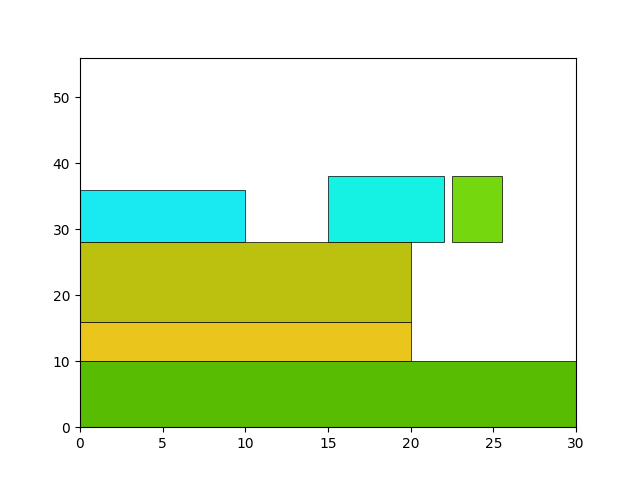
\includegraphics[scale=0.5]{../examples/original-2.png}
            \caption{Example \ref{ex2}, original Steinberg algorithm}
        \end{figure} 
    \end{example}
    \begin{example}\label{ex3}
        Let $W = 30$ and 
        \begin{equation*}
            \begin{aligned}
            L = \{&(5, 3),~(5, 3),~(2, 4),~(30, 8),~(10, 20),~(20, 10),~(5, 5),~(5, 5),\\
                  &(10, 10),~(10, 5),~(6, 4),~(1, 10),~(8, 4),~(6, 6),~(20, 14)\}
            \end{aligned}
        \end{equation*} 
        Steinberg’s packing provides $H = 71$. Respective packing is pictured below
        \begin{figure}[H]
            \centering
            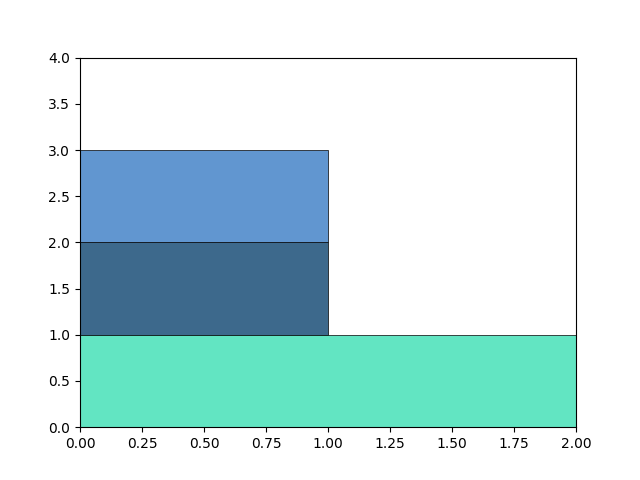
\includegraphics[scale=0.5]{../examples/original-3.png}
            \caption{Example \ref{ex3}, original Steinberg algorithm}
        \end{figure} 
    \end{example}
    \begin{example}\label{ex4}
        Let $W = 12$ and $L = \{(4,3),~(4,9),~(1,12),~(2,3),~(2,7),~(2,2),~(5,2),~(5,6),~(5,4)\}$. We have that $H^{*} = 12$:
        \begin{equation*}
            O^{*}=\{(1,9),~(1,0),~(0,0),~(10,0),~(10,3),~(10,10),~(5,0),~(5,2),~(5,8)\}
        \end{equation*} 
        Steinberg’s packing provides $H = 23.46$. Respective packing is pictured below
        \begin{figure}[H]
            \centering
            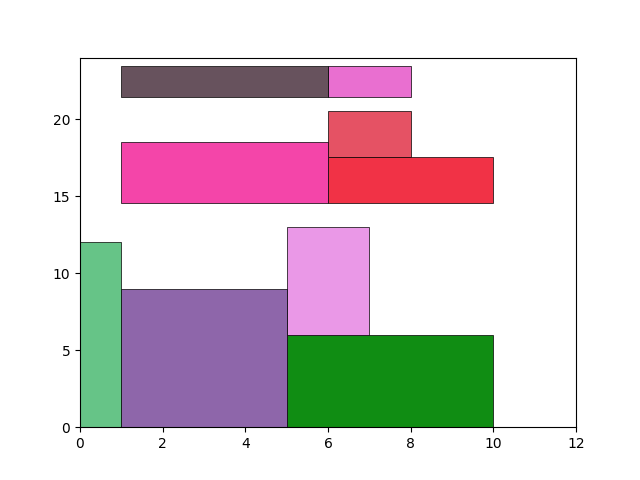
\includegraphics[scale=0.5]{../examples/original-4.png}
            \caption{Example \ref{ex4}, original Steinberg algorithm}
        \end{figure} 
    \end{example}
    \begin{example}\label{ex5}
        Let $W = 25$ and $L = \{(10, 8),~(10, 8),~(12, 4),~(12, 4),~(25, 3)\}$. We have that $H^{*} = 15$:
        \begin{equation*}
            O^{*} = \{(0,0),~(10,0),~(0,8),~(12,8),~(0,12)\}
        \end{equation*}
        Steinberg’s packing provides $H = 23.8$. Respective packing is pictured below
        \begin{figure}[H]
            \centering
            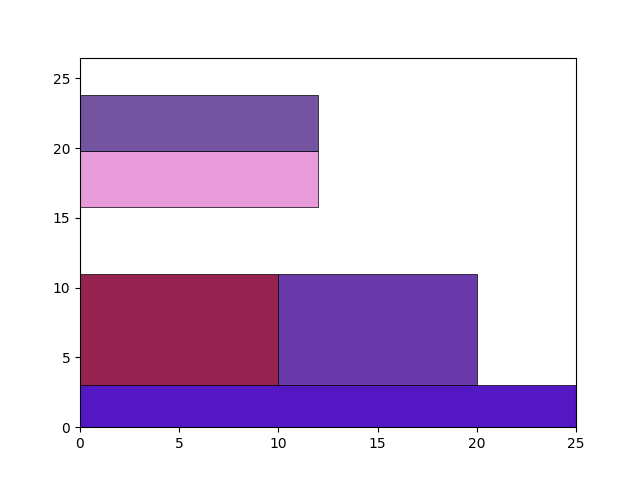
\includegraphics[scale=0.5]{../examples/original-5.png}
            \caption{Example \ref{ex5}, original Steinberg algorithm}
        \end{figure} 
    \end{example}
    \begin{example}\label{ex6}
        Let $W = 10$ and $L = \{(3,3),~(7,2),~(7,1),~(9,3),~(5,4),~(4,4),~(7,1)\}$. We have that $H^{*} = 11$:
        \begin{equation*}
            O^{*}=\{(0,0),~(3,1),~(3,0),~(0,4),~(5,7),~(0,7),~(0,3)\}
        \end{equation*} 
        Steinberg’s packing provides $H = 18$. Respective packing is pictured below
        \begin{figure}[H]
            \centering
            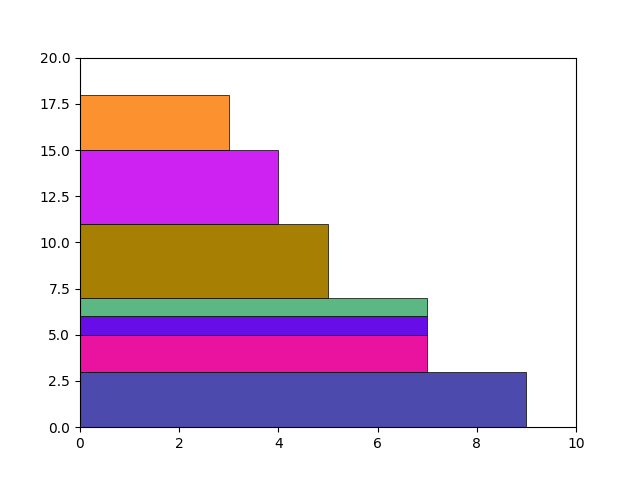
\includegraphics[scale=0.5]{../examples/original-6.png}
            \caption{Example \ref{ex6}, original Steinberg algorithm}
        \end{figure} 
    \end{example}
    \begin{example}\label{ex7}
        Let $W = 10$ and $L = \{(1,1),~(1,1),~(10,8),~(3,1),~(9,1),~(2,1),~(1,1),~(3,1)\}$. We have that $H^{*} = 10$:
        \begin{equation*}
            O^{*}=\{(9,9),~(8,9),~(0,0),~(5,9),~(0,8),~(3,9),~(9,8),~(0,9)\}
        \end{equation*} 
        Steinberg’s packing provides $H = 18.25$. Respective packing is pictured below
        \begin{figure}[H]
            \centering
            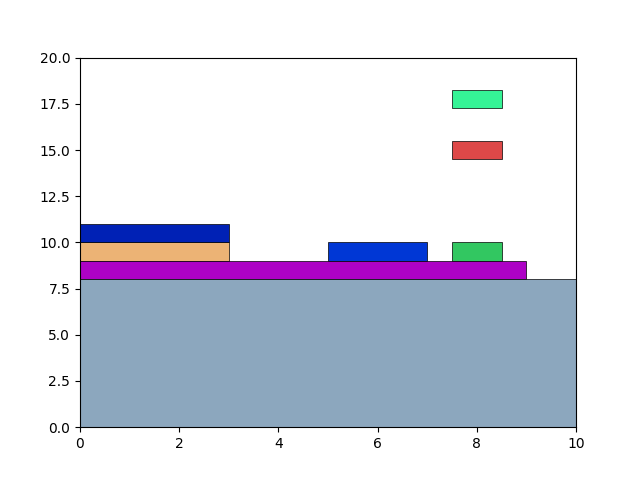
\includegraphics[scale=0.5]{../examples/original-7.png}
            \caption{Example \ref{ex7}, original Steinberg algorithm}
        \end{figure} 
    \end{example}
\section*{Modifications of the Steinberg algorithm}
    As we see in Examples \ref{ex2}--\ref{ex5}, \ref{ex7}, Steinberg’s algorithm provides ”loose” packing. Let us provide two modifications and then analyze them.
    \subsection*{Remove all gaps}
        In Examples \ref{ex4}, \ref{ex5}, \ref{ex7}, we see that the packings involve gaps. Let us remove them. Formally, let 
        \begin{equation*}
            S=\{(x,y)\in\mathbb{Q}^2\mid 0\leq x\leq W,~y\geq0\},~W\in \mathbb{Q}_{+}, 
        \end{equation*}
        and 
        \begin{equation*}
            L={(w_i,h_i)}_{i=1}^{n} \subset \mathbb{Q}_{+}^2,~n\in\mathbb{N}.
        \end{equation*}
        Let $P$ be a packing w.r.t. $L$ and $S$. Let $H = H(P)$. A region $G = [0;W]\times[y_1;y_2]\cap Q^2$ is said to be a \textit{gap} if $[y_1;y_2] \subset [0;W]\times [0;H]$ and ${\rm Int}(R_i)\cap G = \varnothing$, for every $i$, $1 \leq i \leq n$.

        $C = \{R\}_{i\in I}$, $I \subset \{1,\dots,n\}$, is said to be a \textit{component} if, for any pair $i,j \in I$, there exists $i_1,\dots,i_k \in I$ such that
        \begin{equation*}
            \begin{aligned}
                &[y_i;y_i+h_i]\cap[y_{i_1};y_{i_1} +h_{i_1}] \neq \varnothing,\\
                &[y_{i_1};y_{i_1} +h_{i_1}]\cap[y_{i_2};y_{i_2} +h_{i_2}]\neq \varnothing,\\
                &\dots~\dots~\dots~\dots~\dots~\dots~\dots~\dots~\dots\\
                &[y_{i_k};y_{i_k} +h_{i_k}]\cap[y_{j};y_{j}+h_{j}]\neq \varnothing
            \end{aligned}
        \end{equation*} 
        Let $y_0^C = \displaystyle\min_{i\in I} y_i$ and $y_1^C = \displaystyle\max_{i\in I} y_i + h_i$ be the ''bottom'' and ''top'' of a component $C$.

        The ''removing gaps'' procedure involves the following steps:
        \begin{enumerate}
            \item
                We initialize the list of lists $\{\{R_1\}, . . . \{R_n\}\}$.
            \item
                While it is possible, we merge lists if they form a component.
            \item
                After Step 2, we have a list $\{C\}$ of maximal components. We order and re-number this list by increasing the ''bottoms''. We successively lower the components down so that the ''top'' of a component coincides with the ''bottom'' of the next component.
        \end{enumerate}
        The time complexity of this procedure is not greater than $O(n^2)$. For Examples \ref{ex4}, \ref{ex5} and \ref{ex7}, we obtain reduced heights $H = 21$, $H = 19$ and $H = 13$ respectively. Let us again picture modified packing.
        \begin{figure}[H]
            \centering
            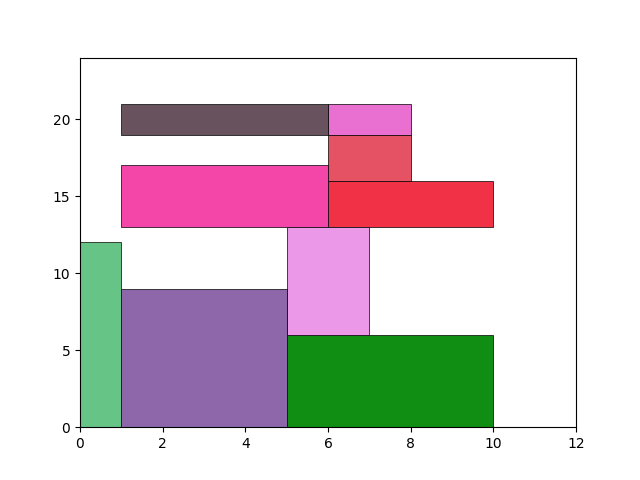
\includegraphics[scale=0.5]{../examples/no-gaps-4.png}
            \caption{Example \ref{ex4}, gaps removed}
        \end{figure}
        \begin{figure}[H]
            \centering
            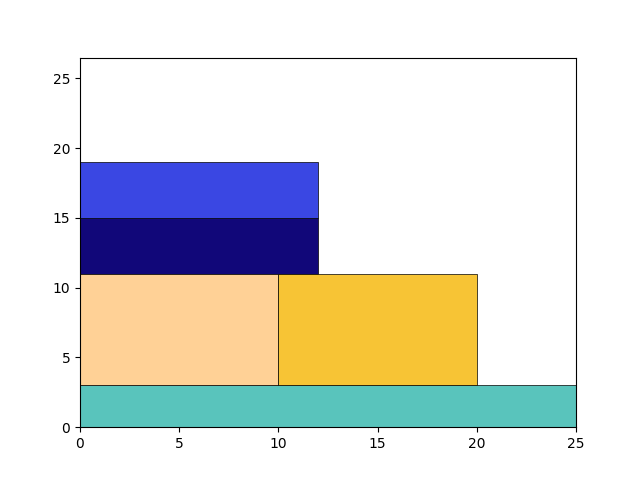
\includegraphics[scale=0.5]{../examples/no-gaps-5.png}
            \caption{Example \ref{ex5}, gaps removed}
        \end{figure} 
        \begin{figure}[H]
            \centering
            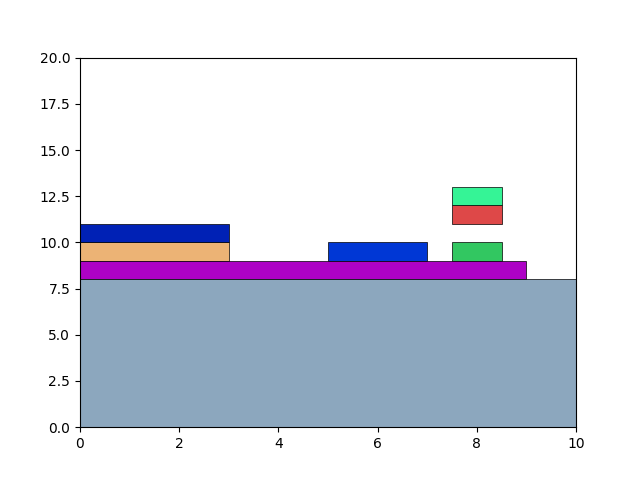
\includegraphics[scale=0.5]{../examples/no-gaps-7.png}
            \caption{Example \ref{ex7}, gaps removed}
        \end{figure}
    \subsection*{Drop hanging rectangles}
        Previous modification could be improved. For instance, in Example \ref{ex2}, it does nothing. Let us ''drop'' all hanging rectangles. Formally, let 
        \begin{equation*}
            S=\{(x,y)\in\mathbb{Q}^2\mid 0\leq x\leq W,~y\geq0\},~W\in\mathbb{Q}_{+},
        \end{equation*}
        and
        \begin{equation*}
            L=\{(w_i,h_i)\}_{i=1}^{n}\subset\mathbb{Q}^2_{+},~n\in\mathbb{N}.
        \end{equation*}
        Let $P$ be a packing w.r.t. $L$ and $S$. For each rectangle $R_i$, $1\leq i\leq n$, let us define the downstrip
        \begin{equation*}
            S_i:=[x_i;x_i+w_i]\times[0;y_i].
        \end{equation*}
        $R_i$ is said to be \textit{hanging} if one of the conditions holds
        \begin{enumerate}
            \item
                $S_i\in {\rm Int}(R_j)=\varnothing$, for every $j\neq i$, and $y_i>0$.
            \item
                There exists $j\neq i$ such that $S_i\cap{\rm Int}(R_j)\neq\varnothing$ and
                \begin{equation*}
                    y_i > \max\{y_j + h_j \mid j\neq i,~S_i\cap {\rm Int}(R_j)\neq\varnothing\}
                \end{equation*}
        \end{enumerate}
        If $R_i$ is hanging, let us denote
        \begin{equation*}
            \eta_i := \begin{cases}
                0 &\text{condition 1 holds}\\
                \max\{y_j + h_j \mid j\neq i,~S_i\cap{\rm Int}(R_j)\neq\varnothing\} &\text{otherwise}
            \end{cases}
        \end{equation*}
        Therefore, \textit{to drop} $R_i$ means that we replace $y_i$ with $\eta_i$.

        The "dropping rectangles" procedure is to sequentially drop hanging rectangles as long as possible.

        The time complexity of this procedure is not greater than $O(n^2)$. 

        For Examples \ref{ex2}--\ref{ex5} and \ref{ex7}, it provides the heights: $38$, $71$, $21$, $19$ and $12$. For Example \ref{ex7}, this modification provides better result than the "removing gaps" modification does. Let us picture an implementation of the modification to Examples \ref{ex2}--\ref{ex4}, \ref{ex7}.
        \begin{figure}[H]
            \centering
            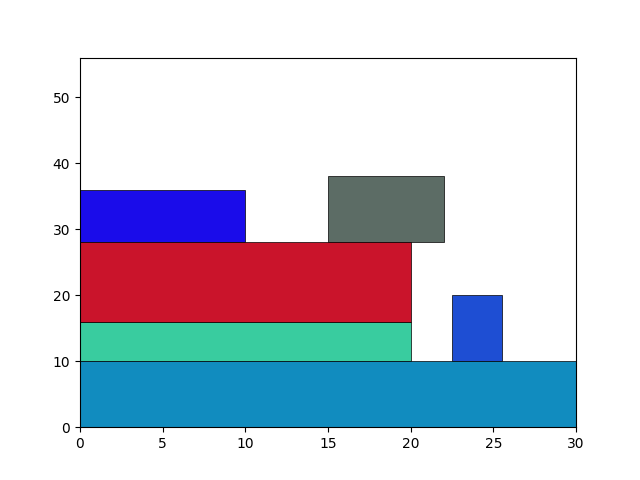
\includegraphics[scale=0.5]{../examples/dropped-2.png}
            \caption{Example \ref{ex2}, rectangles dropped}
        \end{figure}
        \begin{figure}[H]
            \centering
            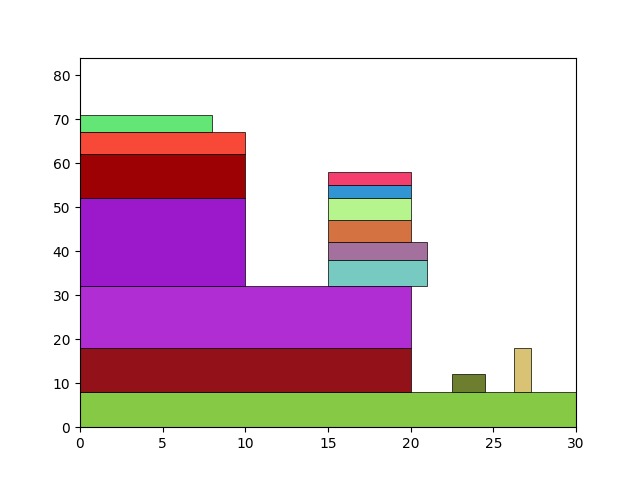
\includegraphics[scale=0.5]{../examples/dropped-3.png}
            \caption{Example \ref{ex3}, rectangles dropped}
        \end{figure}
        \begin{figure}[H]
            \centering
            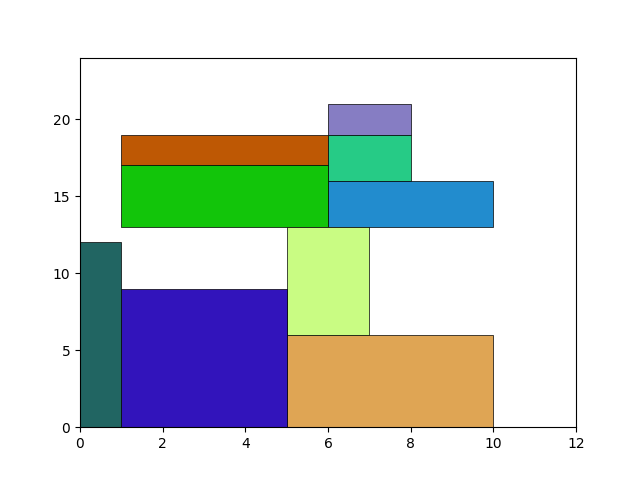
\includegraphics[scale=0.5]{../examples/dropped-4.png}
            \caption{Example \ref{ex4}, rectangles dropped}
        \end{figure}
        \begin{figure}[H]
            \centering
            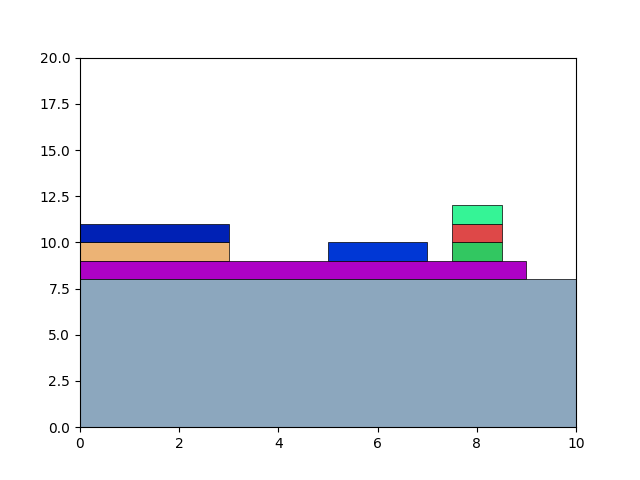
\includegraphics[scale=0.5]{../examples/dropped-7.png}
            \caption{Example \ref{ex7}, rectangles dropped}
        \end{figure}
\section*{Tests}
    Let us compare the Steinberg algorithm, the "removing gaps" and the "dropping hanging rectangles" modifications on random data. We consider two scenarios 
    \begin{enumerate}
        \item\textbf{Test with the predefined optimal height}

        Let us take random values $10\leq W$, $H\leq 100$ and $3\leq n\leq 100$. Then we cut $n$ times (if possible) a rectangle of width $W$ and height $H$ into smaller rectangles. The cuts are also random: we choose a random orientation (horizontal or vertical) and then cut in a random place. Thus, we obtain a strip of width $W$ and a list of rectangles $L$ with predefined optimal height $H$ (''simply connected packing'').
        
        \item\textbf{Test without the predefined optimal height}

        Let us take random values $3\leq W\leq 100$ and $3\leq n\leq 100$. Then we take $n$ times random values $1\leq w\leq W$ and $1\leq h\leq 100$. Thus, we obtain a strip of width $W$ and a list of rectangles $L$ with unknown optimal height.
    \end{enumerate}
    The Steinberg algorithm, the ''removing gaps'' and the ''dropping rectangles'' modifications were tested for $N = 10000$ random examples, for each of the scenarios.

    We consider the statistics
    \begin{itemize}
        \item
            Average approximation ratio $\alpha_0$: let $H_K$ be the height obtained for Example $K$, and $H^{*}_K$ be respective optimal height, $1\leq K\leq N$. Then
            \begin{equation*}
                \alpha_0:=\frac{1}{N}\sum_{K=1}^{N}\frac{H_K}{H^{*}_K}
            \end{equation*}
        \item
            Modification success frequency $\omega$ and average efficiency $\delta$: let $\mathcal{K}$ be the set of examples for which the modification provides better height ${H'}_K$ than the original algorithm does (i.e. ${H'}_K < H_K$). Then
            \begin{equation*}
                \omega=\frac{{\rm card}(\mathcal{K})}{N},~\delta=\frac{1}{{\rm card}(\mathcal{K})}\sum_{K\in\mathcal{K}}\frac{H_K}{{H'}_{K}}
            \end{equation*}
        \item
            Average specific time $\tau$: let $n_K$ be the count of rectangles and $t_K$ be the execution time (in seconds) for Example $K$. Then
            \begin{equation*}
                \tau = \frac{1}{N}\sum_{K=1}^{N}\frac{t_K}{n_K}
            \end{equation*}
    \end{itemize}
    \begin{table}[H]
        \begin{center}
            \begin{tabular}{|c|c|c|c|c|} 
                 \hline
                  & $\alpha_0$ & $\omega$ & $\delta$ & $\tau$ \\  
                 \hline
                 original & $1.921$ & -- & -- & $10^{-5}$ \\ 
                 \hline
                 removing gaps & $1.872$ & $0.556$ & $1.051$ & $10^{-4}$ \\
                 \hline
                 dropping rectangles & $1.692$ & $0.815$ & $1.178$ & $10^{-4}$ \\
                 \hline
            \end{tabular}
            \caption{Results of scenario 1}
        \end{center}
    \end{table}
    \begin{table}[H]
        \begin{center}
            \begin{tabular}{|c|c|c|c|c|} 
                 \hline
                  &  $\omega$ & $\delta$ & $\tau$ \\  
                 \hline
                 original  & -- & -- & $10^{-5}$ \\ 
                 \hline
                 removing gaps & $0.392$ & $1.166$ & $10^{-4}$ \\
                 \hline
                 dropping rectangles  & $0.461$ & $1.201$ & $10^{-4}$ \\
                 \hline
            \end{tabular}
            \caption{Results of scenario 2}
        \end{center}
    \end{table}
\section*{Conclusion}
    Due to the complexity of direct algorithms, we have to use approximating algorithms, which provide non-optimal solutions but are still acceptable. It is worth highlighting the algorithms with an upper estimate for the ratio between heights. We considered in this paper the Steinberg algorithm and proposed two modifications: removing gaps and dropping rectangles. It is noticeable that being more efficient, they both run in an adequate time. When the ''simple connected'' packing exists, dropping rectangles provides an average ratio of $1.692$ and works in $> 80\%$ of cases. In the case of more general packing, it is $1.2$ times better than the original algorithm and works in $> 45\%$ of cases.
\bibliographystyle{unsrtnat}
\begin{thebibliography}{1}
    \bibitem{bakercoffmanrivest} 
        B. S. Baker, E. G. Coffman Jr., R. L. Rivest.
        \newblock Orthogonal Packings in Two Dimensions.
        \newblock {\it SIAM J. Comput.}, 9(4):846--855, 1980.
    \bibitem{lodimartellomonaci} 
        A. Lodi, S. Martello, M. Monaci.
        \newblock Two-dimensional packing problems: A survey.
        \newblock {\it Eur. J. Oper. Res.}, 141:241--252, 2002.
    \bibitem{steinberg} 
        A. Steinberg.
        \newblock A strip-packing algorithm with absolute perfomance bound $2$.
        \newblock {\it SIAM J. Comput.}, 26(2):401--409, 1997.
    \bibitem{jansenrau} 
        K. Jansen, M. Rau.
        \newblock Closing the Gap for Pseudo-Polynomial Strip Packing.
        \newblock {\it 27th Annual European Symposium on Algorithms (ESA 2019)}, 144(62):1--14, 2019.
\end{thebibliography}
\end{document}






